\documentclass[12pt, a4paper]{article}
\usepackage[utf8]{inputenc}
\usepackage{amsmath}
\usepackage{graphicx}


\def\separator{\begin{center}    \rule{100pt}{0.5pt}\end{center}}

\setlength{\parindent}{0em}
\setlength{\parskip}{1em}



\begin{document}

\section{INTRODUZIONE}
\subsection{Astrazioni}
Per isolare i vari livelli di un computer (hardware, kernel, SO), ogni strato fornisce delle interfacce (o set di istruzioni) con la quale interagire al livello sottostante.
Le più importanti sono:
\begin{itemize}
    \item ISA (Instruction Set Architecture) $\rightarrow$ insieme istruzioni macchina
    \item ABI (Application Binary Interface) $\rightarrow$ interfaccia delle applicazioni
\end{itemize}

\subsection{prestazioni}
Le prestazioni si misurano con il \textbf{tempo di esecuzione di un programma} che è composto da 3 variabili:
\textbf{numero di istruzioni}, \textbf{cicli di clock per istruzione} e \textbf{frequenza di clock}
\begin{center}
    tempo di CPU = $\frac{numero\ istruzioni\ \times \ CPI}{frequenza\ di\ clock}$
\end{center}

\subsection{ISA}
 - influisce direttamente sul tempo di cpu (un isa è progettata per frequenze di clock più spinte, è esplicitato il numero di cicli per un'instruzione, e il numero di istruzioni stesso per compiere un'operazione)
 le ISA che affronteremo:
 \begin{itemize}
    \item RISC-V (RISC): cloud computing e sistemi embedded
    \item Intel (CISC): PC
    \item ARM (A-RISC): embedded e mobile
 \end{itemize}


\section{ARITMETICA DEI CALCOLATORI}

\subsection{Basi}
 L'aritmetica nei calcolatori viene fatta su base binaria, quindi bisogna eseguire delle conversioni da una base all'altra.
 per un passaggio da decimale a binario, prendo il numero in decimale e calcolo ricorsivamente il modulo di 2, da qui tengo la parte il resto.
 Quando arrivo a 1, il mio numero in binario saranno i resti letti al contrario.
 
 L'addizione in decimale e binario rimane uguale, mentre le moltiplicazioni seguono questo algoritmo: per ogni 0 del moltiplicatore
 mi sposto di un posto a sinistra, mentre con un 1 copio il moltiplicando. Alla fine addiziono tutto.

\subsection{Codifica}
\subsubsection{Numeri negativi}
Esistono 3 metodi per rappresentare i numeri negativi: \textbf{modulo e segno}, \textbf{complemento a 1}, \textbf{complemento a 2}. 
Con tutti questi metodi, il bit più a sinistra rappresenta il segno

\textbf{modulo e segno:} il più semplice, con il bit più a sinistra rappresenta il segno (1 per -, 0 per +)

\textbf{complemento a 1:} un numero positivo viene rappresento come valore assoluto, mentre uno negativo
 lo rappresento con complimento a 1. \\
    I metodi del complemento sono 2:\\
    - cambio tutti i bit da 1 a 0 e da 0 a 1\\
    - sottraggo il numero a un numero della stessa lunghezza con tutti i bit a 1 
    (11111 - 00101 = 11010)
   
\textbf{Somma e sottrazione con complemento a 1:}
    i numeri negativi li rappresento con complemento a 1 e poi sommo i 2 numeri.Il riporto sul bit più significativo
    lo sommo al risultato. 
    \begin{center}
         6-3 $\rightarrow$ 6 + (-3) $\rightarrow$ 00110 + 11100 $\rightarrow$ 00010 con riporto di 1 $\rightarrow$
         00010 + 1 = 00011 = 3
    \end{center}

\textbf{complemento a 2:}
per eseguire un complemento a 2 si possono usare 3 metodi:
\\ - metodo 1: dato un numero trovo il primo bit a 1 partendo da destra, poi eseguo il complemento a 1 per tutti i bit successivi
\\ - metodo 2: eseguo il complemento a uno del numero, e poi addiziono 1
\\ - metodo 3: prendo il numero con primo bit di sinistra a 1 e resto a zero e di lunghezza pari al numero che ci interessa, infine sottraggo quest'ultimo

Il complemento a 2 risulta più conveniente per le somme, la codifica dello zero è unica e nell'operazione inversa, infatto per eseguire quest'ultima
si osserva il primo bit. Se è pari a 0, allora converto normalmente, se no eseguo il complemento a 2 e sommo 1, poi converto in base 10
\\Il vantaggio con il complemento a 2 si guadagna un valore negativo. Sfortunatamento però si posson oanche generare degli overflow.
Bisogna sempre controllare se da somma di positiva risulta in negativo o se da somma di negativi risulta un positivo
 


\subsubsection{Rappresentazione numeri reali}
\textbf{virgola fissa}
  - si dedica una parte della stringa di bit come parte intera e parte frazionaria
  - genericamente trattiamo il numero come intero e poi moltiplichiamo per -n (dove n rappresenta le cifre decimali)
  - non ci sono errori di approsimazione, ma risulta difficile gestire numeri particolarmente grandi o piccoli
  - per la conversione della parte decimale moltiplico per 2 e considero le parti intere

\textbf{virgola mobile}
  - un numero reale viene suddiviso come mantissa ed esponente
\newpage
\subsection{Codifica del testo}
\subsubsection{ASCII}
\marginpar{NB: 0x denota l'utilizzo di codifica esadecimale}
Per la codifica del testo si usa l'Ascii (American Standard Code for Information Interchange).
Ci sono 2 versioni: ASCII
e ex-ASCII (o ASCII extendend). La differenza tra i due è che il primo uso 7 bit per la codifica, mentre il secondo usa anche il bit significativo
Il bit significativo del ex-ASCII, espande nuove lettere in base al codice del linguaggio 
(8859-1 - caratteri europa occidentale, 8859-5 - cirillico,...). L'extendend inoltre può causare problemi di condivisione data
la sua dipendenza dal codice dei caratteri.\\
Per ulteriori caratteri si utilizza l'unicode o UTF, nelle vari versioni a 32,16 o 8 bit. l'UTF-8 è compatibile con ASCII

\newpage
\section{Reti logiche}
- nei circuiti elettronici, i transistor hanno 2 livelli: uno alto per 1 e uno basso per 0
- le reti logiche sono circuiti che dati valori logici in entrata, ne forniscono altri un uscita
 - possono essere combinatorie, cioé senza memoria e l'uscita dipende solo dal valore in ingresso
 - possono essere sequenziali, cioé hanno memoria e l'uscita dipende anche dai precedenti ingressi
- tabella di verità, espone gli uotput di tutte le combinazioni di input

\subsection{Algebra di Boole}
L'algebra di boole viene utilizzata per le operazioni logiche. gli operatori di base sono l'AND ($\cdot$), l'OR (+) e il NOT ($\overline{A}$)
Come l'algebra matematica, l'algebra di boole possiede delle proprietà
\begin{itemize}
  \item A+0=A, A$\cdot$1=A (identità)
  \item A+1=1, A$\cdot$0=0 (zero e uno)
  \item A+$\overline{A}$=1, A$\cdot$$\overline{A}$=0 (inversa)
  \item A+B=B+A, A$\cdot$B=B$\cdot$A (commutativa)
  \item A+(B+C)=(A+B)+C, A$\cdot$(B$\cdot$C)=(A$\cdot$B)$\cdot$C (associativa)
  \item A$\cdot$(B+C)=(A$\cdot$B)+(A$\cdot$C), A+(B$\cdot$C)=(A+B)$\cdot$(A+C) (distributiva)
\end{itemize}

Due di queste proprietà sono chiamate leggi di De Morgan
\begin{itemize}
  \item $\overline{A\cdot B} = \overline{A} + \overline{B}$
  \item $\overline{A+B} = \overline{A}\cdot\overline{B}$
\end{itemize}
Queste ultime due proprietà introducono il NAND (NOT AND) e il NOR (NOT OR)
\begin{center}
  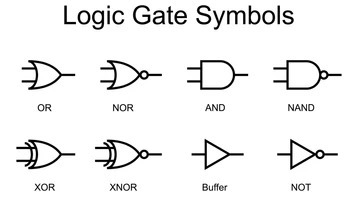
\includegraphics[width=300px]{images/logicGates.jpg}
\end{center}

\subsection{PLA (Programmable Logic Array)}
La PLA è una struttura formata da un barriera di AND (mintermini) e una barriera di OR.\\
Le funzione logiche hanno un costo rappresentato dal numero di porte e ingressi nella rete. 
Il costo può essere ridotto tramite metodi di tipo sistematico o grafico e si riuniscono sotto la "sintesi logica" 

\newpage
\subsection{Reti sequenziali}
Generalmente discutiamo di reti logiche dove in un istante viene dato un output, e nell'istante successivo
quell'output fa parte dei parametri in input. Ma dato che  i segnali richiedono tempo per propagarsi, questo
può causare errori, allora si utilizza il clock per temporizzare le azioni.\\
L'elemento base di memoria è chiamato \textbf{latch} (è composto da due porte NOR). I latch temporizzati vengono chiamati
\textbf{gated latch}. quest'ultimi sono controllati tramite 2 AND sugli ingressi di set e reset 

\begin{center}
  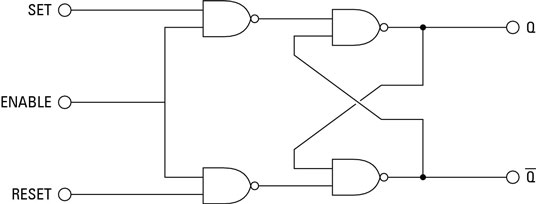
\includegraphics[width=250px]{images/gatedLatch.jpg}
\end{center}

I latch però soffrono l'inconveniente di poter ricevere un 1 sia in set che in reset. Per risolvere il problema del 
doppio 1 si usufruisce dei latch-D e flip flop:\\
il \textbf{latch-D} riceve S e R da un unica variabile messa in NOT su R, mentre il \textbf{flip-flop} usufruisce
di due latch e della negazione del clock, andando a separare nel tempo gli input

Questi elementi di memorizzazione strutturano i registri, cioé una serie di latch in grado di memorizzare una
\textbf{word di dati}. Il loro funzionamento avviene al fronte in salita del clock. Questi funzionamenti in base 
al clock vengono definiti come \textbf{edge triggered}, e offrono il vantaggio di rimuovere le situazioni di corse.

\newpage
\section{Assembly}
un programma in assembly è composto da una lista di istruzioni sequenziali con salti. Queste istruzioni si riuniscono
in 3 macrogruppi:
\begin{itemize}
  \item fetch: preleva un'istruzione dalla memoria
  \item decode: decodifica l'istruzione
  \item execute: eseguisce l'istruzione
\end{itemize}

Le istruzioni vengono anche categorizzate come:
\begin{itemize}
  \item operazioni aritmetico logiche
  \item movimenti di dati/assegnazioni di valore
  \item controlli di flusso
\end{itemize}

I dati con la quale lavoriamo sono classificati come \textbf{immediati} (constanti), \textbf{contenuti in registri}
(general purpose/specializzato, da 4 a 64) e \textbf{contenuti in memoria}

Infine, ci sono due tipi di architettura per la gestione dell processore: il \textbf{CISC} e il \textbf{RISC}

\subsection{RISC (Reduced Instruction Set Computer)}
Il RISC è un'architetture volta alla semplificazione dell'implementazione della cpu. Degli esempi di quest'
archittettura sono intel e RISC-V

I comandi per le istruzioni aritmentico-logiche segue il formato $\langle opcode\rangle\ 
\langle dst\rangle, \langle arg1\rangle, \langle arg2\rangle$\\
Mentre per l'accesso alla memoria la sintassi è:
\begin{itemize}
  \item load $\langle reg\rangle,\ \langle mem\ loc\rangle$
  \item store $\langle mem\ loc\rangle,\ \langle reg\rangle$
\end{itemize}



\subsection{CISC (Complex Instruction Set Computer)} 
Quest'architettura si concentra nel semplificare la scrittura dei programmi da parte del programmatore.
Il numero di istruzioni è maggiore, le istruzioni aritmetico logiche hanno operandi e destinazioni in 
memoria, e la sintassi risulta meno regolare.
Un esempio di questa architettura è ARM


\section{Assembly Risc-v}
Adesso esamineremo l'IS (Instruction Set) di RISC-V, un'architettura moderna e open source

\subsection{istruzioni aritmentico logiche}
\begin{quote}
  \center principio di progettazione n.1: 

  la semplicità favorisce la regolarità
\end{quote}

RISC-V prevede soltato istruzioni aritmentiche a 3 operandi:
\marginpar{commenti con \# }
\begin{center}
  a = b + c + d\\
  $\Downarrow$\\
  add a, b, c\\
  add a, a, d\\
\end{center}

Le istruzioni più complicate vanno suddivise in comandi più semplici:
\begin{center}
  a = (b+c)-(d+e)\\
  $\Downarrow$\\
  add t1, b, c \\
  add t2, d, e \\
  sub a, t1, t2\\
\end{center}  
In RISC-V però, gli operandi sono vincolati ad essere registri

\subsubsection{Registri}
\begin{quote}
  \center principio di progettazione n.2:
  
  minori sono le dimensioni, maggiore la velocità
\end{quote}
Operare solo tra registri semplifica e velocizza il progetto dell'hardware. 
Risc-v contiene \textbf{32 registri a 64 bit}, in maniera da ridurre la propagazione dei segnali 
all'interno del processore. Quindi, correggendo l'esempio di prima:
\begin{center}
  a = (b+c)-(d+e)\\
  $\Downarrow$\\
  add x5, x20, x21 \\
  add x6, x22, x23\\
  sub x19, x5, x6\\
\end{center} 
dove a = x19, b = x20, c = x21, d = x22, e = x23, t1 = x5 e t2 = x6.

\subsection{La memoria}
Ovviamente però il numero di registri non basta, per questo vengono usate istruzioni di 
trasferimento dai registri alla memoria (\textbf{store}) e dalla memoria ai registri
(\textbf{load}) 

\end{document}